\chapter{Self-Supervised Learning}
The models trained from large-scale of data, such as the ImageNet dataset, are
widely used as the pre-trained models and fine-tuned for other tasks for two main
reasons:
\begin{itemize}
      \item The parameters learned from large-scale diverse datasets provide a
            good starting point, therefore, networks training on other tasks can
            converge faster;
      \item The network trained on large-scale datasets already learned the hierarchy
            features which can help to reduce over-fitting problem during the
            training of other tasks, especially when datasets of other tasks are
            small, or training labels are scarce.
\end{itemize}

With the sophisticated architectures and large-scale datasets, the performance
of DNNs keeps breaking the state-of-the-arts for many tasks. However, collection
and annotation of large-scale datasets are time-consuming and expensive.

To avoid time-consuming and expensive data annotations, many \textbf{self-supervised}
methods were proposed to learn visual features from large-scale unlabeled images
or videos without using any human annotations.

A popular solution is to propose various pretext tasks for networks to solve. The
networks can be trained by learning objective functions of the pretext tasks and
in the while the features are learned through this process. Thanks to the pretext
tasks, the data are labeled automatically.

The model created using this method can be used as a pre-trained model and applied
to the supervised downstream tasks to improve the performance.

Various pretext tasks have been proposed for self-supervised learning including
colorizing gray scale images, image inpainting, playing image jigsaw puzzle, etc.
The pretext tasks share two common properties:

\begin{itemize}
      \item Visual features of images or videos need to be captured by CNNs to
            solve the pretext tasks;
      \item The supervisory signal is generated from the data itself (self-supervision)
            by leveraging its structure.
\end{itemize}

During the self-supervised training phase, a predefined pretext task is designed
for CNNs to solve, and the pseudo labels for the pretext task are automatically
generated based on some attributes of data.

Then the CNN is trained to learn objective functions of the pretext task. As with
training on a labeled dataset, when trained with pretext tasks, the shallower
blocks of CNN focus on the low-level general features such as corners, edges, and
textures, while the deeper blocks focus on the high-level task-specific features
such as objects, scenes, and object parts. Therefore, CNNs trained with pretext
tasks can learn kernels that capture low-level features and high-level features
that are helpful for other downstream tasks.

After the self-supervised training is finished, the learned visual features can
be further transferred to downstream tasks as pre-trained models to improve
performance and overcome over-fitting.

The main advantage of self-supervised learning methods is that they can be easily
scaled to large-scale datasets with very low cost.

We now present the terminology that will be used during this section:
\begin{itemize}
      \item \textbf{Human-annotated label}: labels of data that are manually
            annotated by human workers.
      \item \textbf{Pretext Task}: pre-designed tasks for networks to solve, and
            visual features are learned by learning objective functions of pretext
            tasks. The pretext tasks can be predictive tasks, generative tasks,
            contrasting tasks, or a combination of them. The supervision signal
            for pretext tasks is generated from the data itself based on its structure.
      \item \textbf{Pseudo label}: The labels used in pretext task is referred as
            Pseudo labels which are generated based on the structure of data for
            pretext tasks.
      \item \textbf{Downstream Task}: CV applications that can be used to evaluate
            the quality of features learned by self-supervised learning. These
            applications can greatly benefit from the pre-trained models when training
            data are scarce. In general, human-annotated labels are needed to solve
            the downstream tasks. However, in some applications, the downstream task
            can be the same as the pretext task without using any human-annotated
            labels.
      \item \textbf{Supervised Learning}: refers to learning methods using data with
            fine-grained human annotated labels to train networks.
      \item \textbf{Semi-supervised Learning}: refers to learning methods using a
            small amount of labeled data in conjunction with a large amount of
            unlabeled data.
      \item \textbf{Weakly-supervised Learning}: refers to learning methods to learn
            with coarse-grained labels or inaccurate labels. The cost of obtaining
            weak supervision labels is generally much cheaper than fine-grained
            labels for supervised methods.
      \item \textbf{Unsupervised Learning}: refers to learning methods without using
            any human-annotated labels.
      \item \textbf{Self-supervised Learning}: refers to learning methods in which
            CNNs are explicitly trained with supervisory signals that are generated
            from the data itself (self-supervision) by leveraging its structure.
\end{itemize}

We can compare the performance of image feature training by evaluating the
classificator on the same dataset.
\begin{note}
      Self supervised learning add robustness to model.
\end{note}
\section{Learning visual features from pretexts tasks}
To relieve the burden of large-scale dataset annotation, a pretext task is generally
designed for networks to solve while pseudo labels for the pretext task are
automatically generated based on data attributes. Effective pretext tasks are
those ensuring that semantic features are learned through the process of accomplishing
the pretext tasks.

As we have seen before, there are different types of pretext task that can be used
to train a neural network with self supervised learning. We can classify them
into four categories as shown in Figure \ref{fig:SSL}.

\begin{figure}[!ht]
      \centering
      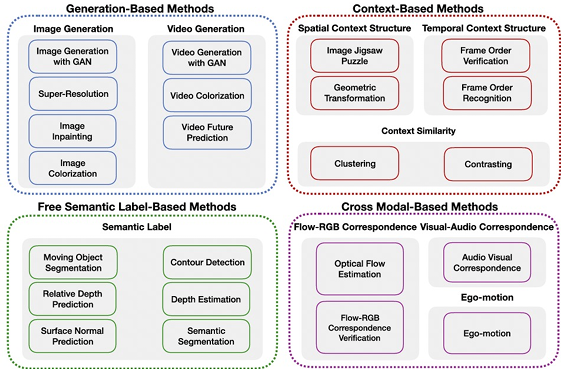
\includegraphics[width=0.5\textwidth]{img/SSL/commonlyPreText.png}
      \caption{Commonly used pretext tasks.}
      \label{fig:SSL}
\end{figure}

\subsection{Generation-based pretext tasks}
This type of methods learn visual features by solving pretext tasks that involve
image or video generation.
\begin{itemize}
      \item \textbf{Image Generation}: Visual features are learned through the
            process of image generation tasks. This type of methods includes image
            colorization, image super resolution, image inpainting, image generation
            with Generative Adversarial Networks (GANs).
      \item \textbf{Video Generation}: Visual features are learned through the
            process of video generation tasks. This type of methods includes video
            generation with GANs, and video prediction.
\end{itemize}

For GAN we train the network and we use only the discriminator and we take features
from last layers.

Generation-based self-supervised methods for learning image features involve the
process of generating images. For these tasks, pseudo training labels $P$ usually
are the images themselves and no human annotated labels are needed during training,
therefore, these methods belong to self-supervised learning methods.

The pioneer work about the image generation-based methods is the Autoencoder which
learns to compress an image into a low-dimension vector and then is uncompressed
into an image that is close to the original image with a bunch of layers.
\subsection{Context-based pretext tasks}
The design of context-based pretext tasks mainly employs the context features of
images or videos such as context similarity, spatial structure, temporal structure,
etc. as the supervision signal.
\begin{itemize}
      \item \textbf{Context Similarity}: Pretext tasks are designed based on the
            context similarity between image patches. This type of methods includes
            image clustering-based methods, and graph constraint-based methods.
            There are two ways of utilizing context similarity as supervision
            signals for self-supervised learning: formulating it as a \textbf{
                  predictive task} or a \textbf{contrastive task}.

            For both methods, the data are first clustered into different groups
            under the assumption that data from the same group have high context
            similarity, while data from different groups have low context similarity.
            \begin{itemize}
                  \item \textbf{Predictive Task}. The predictive tasks involve
                        training networks to predict the group ID of the data,
                        usually with a cross entropy loss. In this context, the
                        clustering methods are mainly employed as a tool to cluster
                        image data.

                        After the clustering, several clusters are obtained while
                        the image within one cluster have a smaller distance in
                        feature space and images from different clusters have a
                        larger distance in feature space.

                        The smaller the distance in feature space, the more
                        similar the image in the appearance in the RGB space.

                        Then a CNN can be trained to classify the data by using
                        the cluster assignment as the pseudo class label. To
                        accomplish this task, the CNN needs to learn the invariance
                        within one class and the variance among different classes.
                        Therefore, the CNN learns semantic meaning of images.
                  \item \textbf{Contrastive Task}. The contrastive tasks involve
                        training networks to directly minimize feature distances
                        from the same group and maximize feature distances from
                        different groups, usually with a triplet loss or a
                        contrastive loss.

                        The general idea of the contrastive SSL is to train networks
                        to maximum agreement of different views of same scene
                        while minimizing agreement of views from different
                        scenes.

                        The recent state-of-the-art method is SimCLR which learns
                        features by contrasting images after a composition of data
                        augmentations. The positive pairs are constructed by
                        sampling two images after applying different augmentation
                        techniques for the same image, while negative pairs include
                        two different images.
            \end{itemize}
      \item \textbf{Spatial Context Structure}: Pretext tasks used to train CNNs
            are based on the spatial relations among image patches. This type of
            methods includes image jigsaw puzzle, context prediction, and geometric
            transformation recognition, etc.

            The pretext task can be to predict the relative positions of two patches
            from same image, or to recognize the order of a shuffled sequence of
            patches from same image. The context of full images can also be used
            as a supervision signal to design pretext tasks such as to recognize
            the rotating angles of the whole images. To accomplish these pretext
            tasks, CNNs need to learn spatial context information such as the shape
            of the objects and the relative positions of different parts of an
            object.

            \begin{figure}[!ht]
                  \centering
                  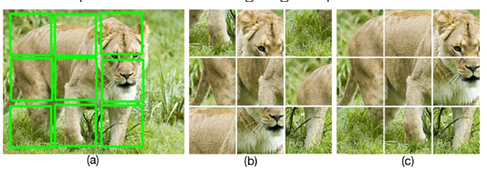
\includegraphics[width=0.5\textwidth]{img/SSL/puzzle.png}
                  \caption{Spatial context structure-based pretext tasks.}
                  \label{fig:SCS}
            \end{figure}

            To limit the number of permutations, usually, Hamming distance is 
            employed to choose only a subset of permutations among all the 
            permutations, i.e., those with a relative large Hamming distance. 
            Only the selected permutations are used to train CNN to recognize the 
            permutation of shuffled image patches.
      \item \textbf{Temporal Context Structure}: The temporal order from videos
            is used as supervision signal. The CNN is trained to verify whether
            the input frame sequence in correct order, or to recognize the order
            of the frame sequence.
\end{itemize}

Features are learned by CNN through the process of solving the pretext tasks
designed based on attributes of the context of images.

\subsection{Free semantic label-based pretext tasks}
This type of pretext tasks train networks with automatically generated semantic
labels. Generally, the free semantic labels such as segmentation masks, depth
images, optical flows, and surface normal images can be rendered by game engine
or generated by hard-code methods.

Since these semantic labels are automatically generated, the methods using the
synthetic datasets or using them in conjunction with a large unlabeled image or
video datasets are considered as self-supervised learning methods.

\begin{note}
      Strictly speaking, the methods based on data generated by game engines
      do/should not belong to the self-supervised learning methods since human
      intervention is needed during the data generation process. However, some
      recent work treat them as self-supervised learning methods.
\end{note}

Game engines can generate realistic images with accurate pixel-level labels with
very low cost. However, due to the domain gap between synthetic and real-world
images, the CNNs purely trained on synthetic images cannot be directly applied
to real-world images. To utilize synthetic datasets for self-supervised feature
learning, the domain gap needs to be explicitly bridged.

To overcome the problem, unsupervised feature space domain adaptation methods
based on adversarial learning have been proposed. The CNN predicts surface normal,
depth, and instance contour for the synthetic images and a discriminator network
$D$ is employed to minimize the difference of feature space domains between
real-world and synthetic data.

\begin{figure}[!ht]
      \centering
      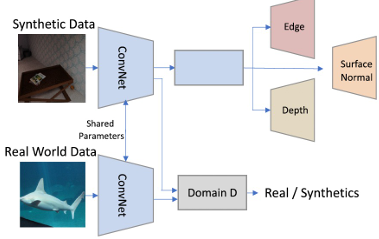
\includegraphics[width=0.5\textwidth]{img/SSL/FreeSemantic.png}
      \caption{Free semantic labels-based pretext tasks.}
      \label{fig:FSL}
\end{figure}

Applying hard-code programs is another way to automatically generate semantic
labels such as salience, foreground masks, contours, depth for images and videos.
With these methods, very large-scale datasets with generated semantic labels can
be used for self-supervised feature learning. This type of methods generally has
two steps:
\begin{enumerate}
      \item Label generation by employing hard-code programs on images or videos
            to obtain labels;
      \item Train CNNs with the generated labels.
\end{enumerate}

No matter what kind of labels used to train CNNs, the general idea of this type
of methods is to distill knowledge from the hard-code detector.

One drawback is that the semantic labels generated by hard-code detector usually
are very noisy which need to be specifically coped with.

\subsection{Cross modal-based pretext tasks}
This type of pretext tasks trains CNNs to verify whether two different channels
of input data are corresponding to each other such as Visual-Audio Correspondence
Verification, RGB-Flow Correspondence Verification, Contrasting (i.e., maximizing
agreement between differently augmented views of the same data example), and egomotion.

\begin{center}
      Egomotion is defined as the 3D motion of a camera within an environment.
      In the field of computer vision, egomotion refers to estimating a camera's
      motion relative to a rigid scene. An example of egomotion estimation would
      be estimating a car's moving position relative to lines on the road or street
      signs being observed from the car itself. The estimation of egomotion is
      important in autonomous robot navigation applications.
\end{center}

Cross modal-based learning methods usually learn features from the correspondence
of multiple data streams.

In addition to rich temporal and spatial information in videos, optical flow
sequence can be generated to specifically indicate the motion in videos, and the
difference of frames can be computed with negligible time and space-time complexity
to indicate the boundary of the moving objects.

Based on the type of data used, these methods fall into three groups:
\begin{itemize}
      \item Methods that learn features by using the RGB and optical flow
            correspondence;
      \item Methods that learn features by utilizing the video and audio correspondence
      \item Ego-motion that learn by utilizing the correspondence between egocentric
            video and egomotorsensor signals.
\end{itemize}

Usually, the network is trained to recognize if the two kinds of input data are
corresponding to each other, or is trained to learn the transformation between
different modalities.
\section{Commonly used downstream tasks for evaluation}
To evaluate the quality of the learned image or video features by self-supervised
methods, the learned parameters by SSL are employed as pre-trained models and then
fine-tuned on downstream tasks such as image classification, semantic segmentation,
object detection, and action recognition etc.

The performance of the transfer learning on these high-level vision tasks
demonstrates the generalizability of the learned features.

If CNNs trained in SSL scenarios can learn general features, then the pre-trained
models can be used as a good starting point for other vision tasks that require
capturing similar features from images or videos.

In addition to the quantitative evaluations of the learned features, there are
also some qualitative visualization methods to evaluate the quality of SSL features.
Three methods are often used for this purpose:
\begin{enumerate}
      \item \textbf{Kernel visualization}: Qualitatively visualize the kernels of
            the first convolution layer learned with the pretext tasks and compare
            the kernels from supervised models. The similarity of the kernels
            learned by supervised and self-supervised models are compared to
            indicate the effectiveness of self supervised methods.
      \item \textbf{Feature Map Visualization}: Feature maps are visualized to
            show the attention of networks. Larger activation represents the neural
            network pays more attention to the corresponding region in the image.
            Feature maps are usually qualitatively visualized and compared with
            that of supervised models.
      \item \textbf{Nearest Neighbor Retrieval}: In general, images with similar
            appearance usually are closer in the feature space. The nearest
            neighbor method is used to find the top $K$ nearest neighbors from
            the feature space of the features learned by the self-supervised
            learned model.
\end{enumerate}